\documentclass{beamer}

\usepackage{pgfpages}
%\setbeameroption{show notes}
%\setbeameroption{show notes on second screen=right}
\mode<presentation> {
  \usetheme{Warsaw}
  % ou autre ...

  \setbeamercovered{transparent}
  % ou autre chose (il est également possible de supprimer cette ligne)
}


\usepackage[french]{babel}
\usepackage[latin1]{inputenc}
\usepackage{times}
\usepackage[T1]{fontenc}
\usepackage{tikz}
\usepackage{listings}
\usepackage{color}
\usepackage{graphicx}
\usepackage{multimedia}
\usepackage{media9}
\usetikzlibrary{patterns}
\pgfdeclareimage[height=0.5cm]{le-logo}{}
\logo{\pgfuseimage{le-logo}}
\setbeamertemplate{footline}[frame number]


%%%%%%%%%%%%%%%%%%%%%%%%%%%
\title[Lagrangian Analysis of a 3-Link Planar Robot Arm] 
{Lagrangian Analysis of a 3-Link Planar Robot Arm}
%\subtitle {ne compléter que si l'article possède un sous-titre}

\author{Max A. Feinberg \and Samuel T. Wagner \and Steven P. Schlax }
\institute{\inst{1} University of Illinois Urbana Champaign}

%\institute[]
%{
%  BS Aerospace Engineering, Minor in Computer Science\\
%  University of Illinois Urbana-Champaign
%  \and
%  
\includegraphics[scale=0.5]{NASA}
%  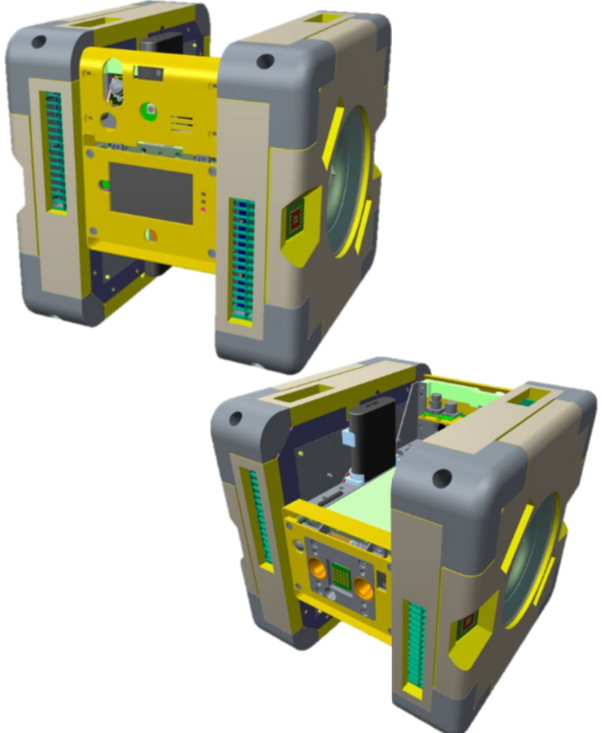
\includegraphics[scale=0.22]{Astrobee}
% 
%  }

\date[SESOS 2015] 


\begin{document}

%{Research Interest: WSAN,Smart Grids,ICT4D}
\newcommand{\nvar}[2]{
    \newlength{#1}
    \setlength{#1}{#2}
}

% Define a few constants for drawing
\nvar{\dg}{0.3cm}
\def\dw{0.25}\def\dh{0.5}
\nvar{\ddx}{1.5cm}

% Define commands for links, joints and such
\def\link{\draw [double distance=1.5mm, very thick] (0,0)--}
\def\joint{%
    \filldraw [fill=white] (0,0) circle (5pt);
    \fill[black] circle (2pt);
}
\def\grip{%
    \draw[ultra thick](0cm,\dg)--(0cm,-\dg);
    \fill (0cm, 0.5\dg)+(0cm,1.5pt) -- +(0.6\dg,0cm) -- +(0pt,-1.5pt);
    \fill (0cm, -0.5\dg)+(0cm,1.5pt) -- +(0.6\dg,0cm) -- +(0pt,-1.5pt);
}
\def\robotbase{%
    \draw[rounded corners=8pt] (-\dw,-\dh)-- (-\dw, 0) --
        (0,\dh)--(\dw,0)--(\dw,-\dh);
    \draw (-0.5,-\dh)-- (0.5,-\dh);
    \fill[pattern=north east lines] (-0.5,-1) rectangle (0.5,-\dh);
}

% Draw an angle annotation
% Input:
%   #1 Angle
%   #2 Label
% Example:
%   \angann{30}{$\theta_1$}
\newcommand{\angann}[2]{%
    \begin{scope}[red]
    \draw [dashed, red] (0,0) -- (1.2\ddx,0pt);
    \draw [->, shorten >=3.5pt] (\ddx,0pt) arc (0:#1:\ddx);
    % Unfortunately automatic node placement on an arc is not supported yet.
    % We therefore have to compute an appropriate coordinate ourselves.
    \node at (#1/2-2:\ddx+8pt) {#2};
    \end{scope}
}

% Draw line annotation
% Input:
%   #1 Line offset (optional)
%   #2 Line angle
%   #3 Line length
%   #5 Line label
% Example:
%   \lineann[1]{30}{2}{$L_1$}
\newcommand{\lineann}[4][0.5]{%
    \begin{scope}[rotate=#2, blue,inner sep=2pt]
        \draw[dashed, blue!40] (0,0) -- +(0,#1)
            node [coordinate, near end] (a) {};
        \draw[dashed, blue!40] (#3,0) -- +(0,#1)
            node [coordinate, near end] (b) {};
        \draw[|<->|] (a) -- node[fill=white] {#4} (b);
    \end{scope}
}

% Define the kinematic parameters of the three link manipulator.
\def\thetaone{30}
\def\Lone{2}
\def\thetatwo{20}
\def\Ltwo{2}
\def\thetathree{40}
\def\Lthree{1}



\begin{frame}
  \titlepage
  \centering
  
\includegraphics[scale = 0.25]{UIUC_logo}
  %\hspace{15mm}
  %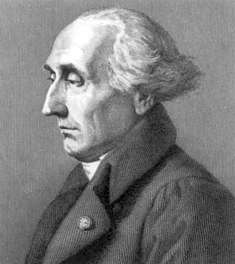
\includegraphics[scale = 0.25]{Lagrange_portrait}
\end{frame}

\begin{frame}{Plan}
  \tableofcontents
\end{frame}


\section{Motivation}
\subsection{But y tho?}
\begin{frame}
\begin{columns}
\column{0.5\textwidth}
\begin{itemize}
\item Robots are awesome and they're the future
\item Analysis of complex robot systems require systematic approaches
\begin{itemize}
\item MIT Cheetah 2 Robot with 34 DOF
\end{itemize}
\end{itemize}

\column{0.5\textwidth}
\begin{figure}
\caption{MIT Cheetah 2}
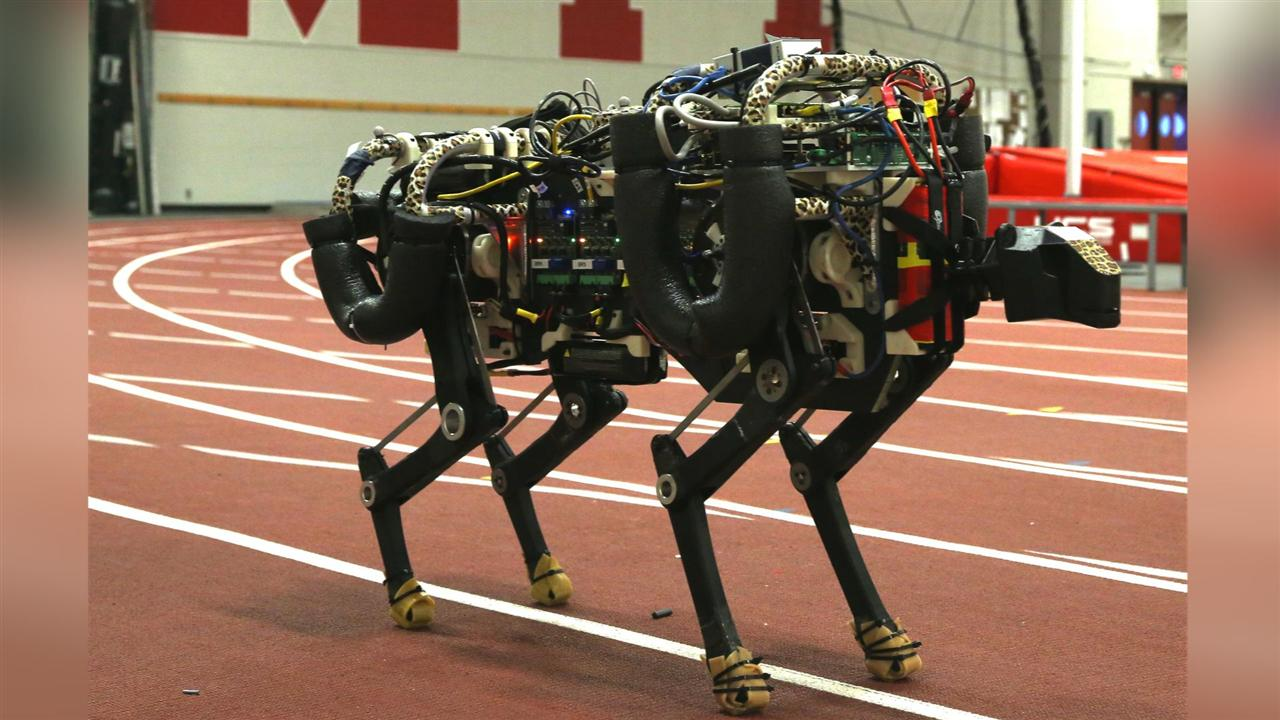
\includegraphics[scale=0.18]{cheetah.jpg}
\end{figure}
\end{columns}

\end{frame}

\begin{frame}

\begin{columns}
\column{0.5\textwidth}
\begin{figure}
	\caption{3-Link Planar Robot Arm}
	\begin{center}
	\begin{tikzpicture}
    \robotbase
    \angann{\thetaone}{$\theta_1$}
    \lineann[0.7]{\thetaone}{\Lone}{$a_1$}
    \link(\thetaone:\Lone);
    \joint
    \begin{scope}[shift=(\thetaone:\Lone), rotate=\thetaone]
        \angann{\thetatwo}{$\theta_2$}
        \lineann[-1.5]{\thetatwo}{\Ltwo}{$a_2$}
        \link(\thetatwo:\Ltwo);
        \joint
        \begin{scope}[shift=(\thetatwo:\Ltwo), rotate=\thetatwo]
            \angann{\thetathree}{$\theta_3$}
            \lineann[0.7]{\thetathree}{\Lthree}{$a_3$}
            \draw [dashed, red,rotate=\thetathree] (0,0) -- (1.2\ddx,0pt);
            \link(\thetathree:\Lthree);
            \joint
            \begin{scope}[shift=(\thetathree:\Lthree), rotate=\thetathree]
                \grip
            \end{scope}
        \end{scope}
    \end{scope}
\end{tikzpicture}
\end{center}
\end{figure}  

\column{0.5\textwidth}
\begin{figure}
\caption{A real "3-Link" Planar Robot Arm}
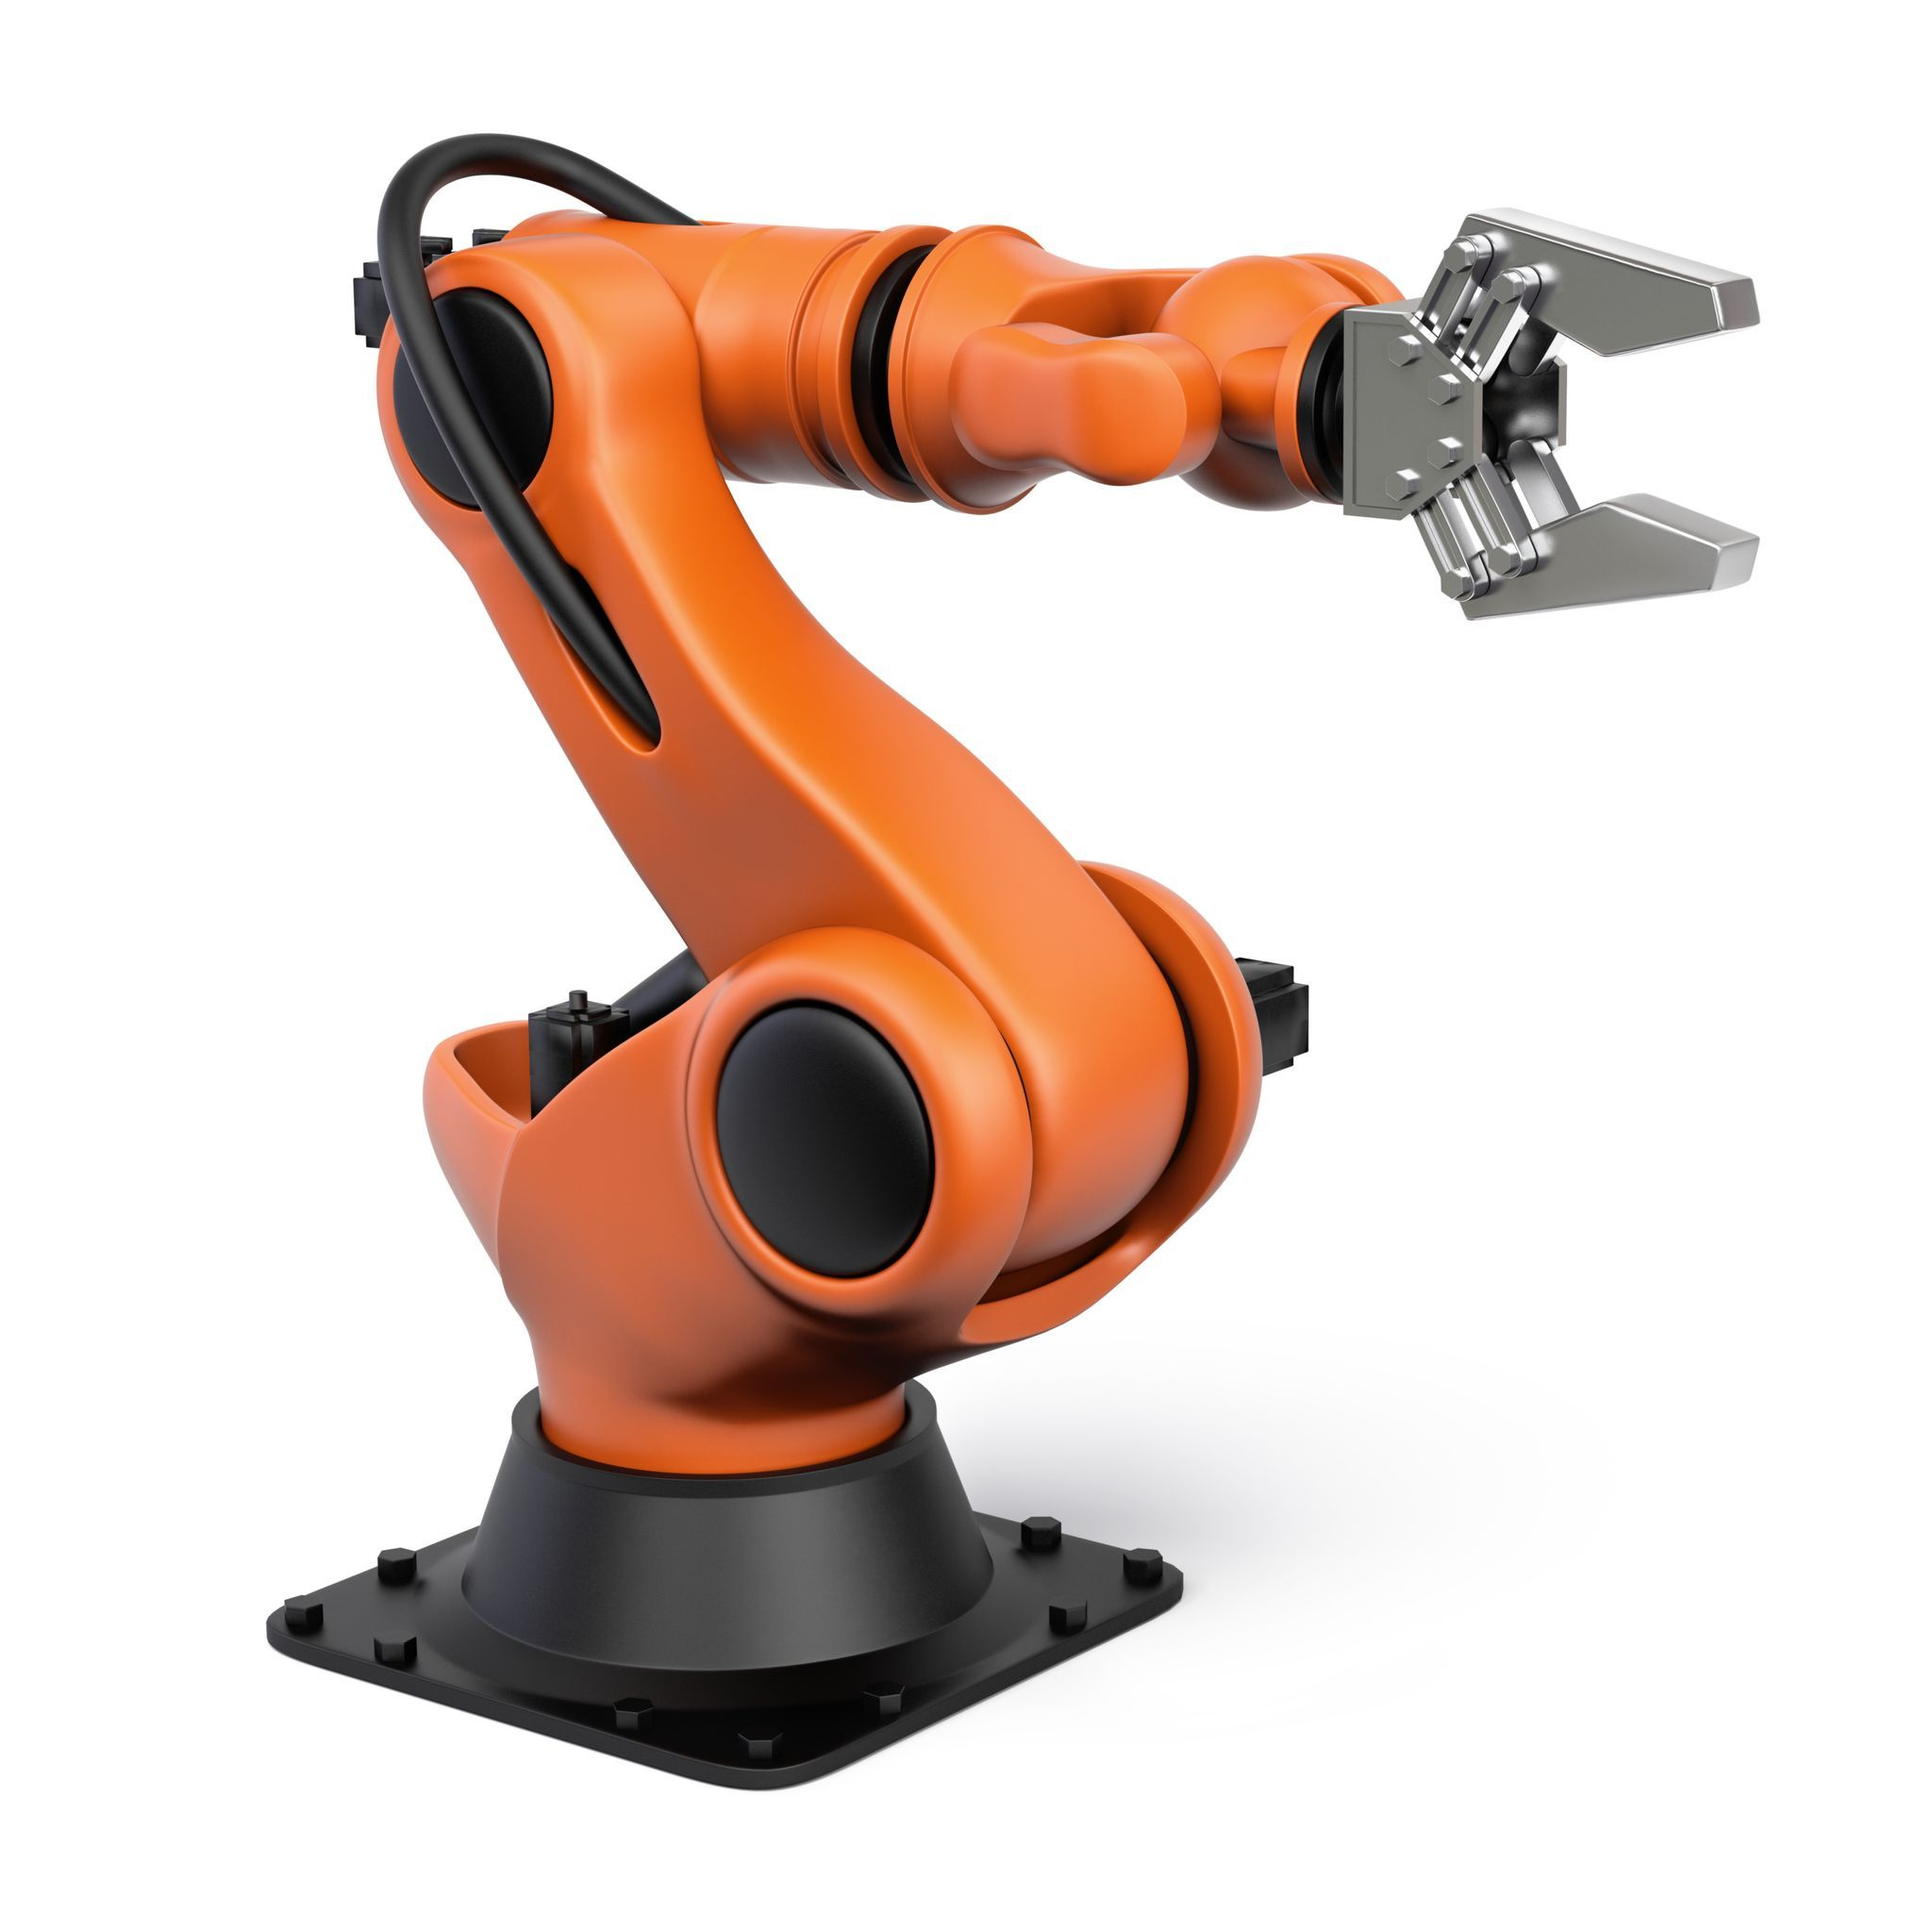
\includegraphics[scale= 0.30]{robot_arm-jpg.jpg}
\end{figure}

\end{columns}

\end{frame}


\section{Approach}
\subsection{Derivation}
\begin{frame}{Important Side Bar}

\begin{block}{The Jacobian}

\begin{eqnarray*}
d\textbf{r}_i & = & \begin{bmatrix}
		\frac{\partial x_i}{\partial q_1} & \dots & \frac{\partial x_i}{\partial q_n}\\
        \frac{\partial y_i}{\partial q_1} & \dots & \frac{\partial y_i}{\partial q_n}\\
        \frac{\partial z_i}{\partial q_1} & \dots & \frac{\partial z_i}{\partial q_n}\\
        \end{bmatrix} 
        \begin{bmatrix}
        dq_1\\
        \vdots\\
        dq_n\\
        \end{bmatrix}\\
d\textbf{r}_i & = & \mathbb{J}_i^L d\textbf{q}\\
\end{eqnarray*} 
\end{block}

\end{frame}

\begin{frame}\frametitle{The Lagrangian Method}
\begin{exampleblock}{The Langrange Equation}
\[
\frac{d}{dt} \Big( \frac{\partial L}{\partial \dot{q}_i} \Big) - \frac{\partial L}{\partial q_i} = Q_i
\]
\end{exampleblock}
\small
\begin{eqnarray*}
T & = & \frac{1}{2} \sum_{i=1}^{n} (m_i v_i^T v_i + w_i^T \mathbb{I}_i w_i)\\
T & = & \frac{1}{2} \sum_{i=1}^{n} (m_i \dot{\textbf{q}}^T (\mathbb{J}_i^L)^T \mathbb{J}_i^L \dot{\textbf{q}} + \dot{\textbf{q}}^T (\mathbb{J}_i^A)^T \mathbb{I}_i \mathbb{J}_i^A \dot{\textbf{q}})\\
T & = & \frac{1}{2} \dot{\textbf{q}}^T \sum_{i=1}^{n} (m_i  (\mathbb{J}_i^L)^T \mathbb{J}_i^L  +(\mathbb{J}_i^A)^T \mathbb{I}_i \mathbb{J}_i^A) \dot{\textbf{q}}\\
T & = & \frac{1}{2} \dot{\textbf{q}}^T \mathbb{H} \dot{\textbf{q}}\\
\end{eqnarray*}
\end{frame}


\begin{frame}\frametitle{The Lagrangian Method}
\begin{exampleblock}{Kinetic Energy Term}
\[
\frac{d}{dt} \Big( \frac{\partial L}{\partial \dot{q}_i} \Big) = \sum_{j=1}^{n} \Big( \sum_{k=1}^{n} \frac{\partial H_{ij}}{\partial q_k} \dot{q}_k \dot{q}_j + H_{ij} \ddot{q}_j \Big)
\]
\end{exampleblock}
\begin{exampleblock}{Potential Energy Term}
\[
\frac{\partial L}{\partial q_i} = - \frac{\partial U}{ \partial q_i}
\]
\end{exampleblock}
\end{frame}

\begin{frame}\frametitle{MATLAB}

\begin{block}{General Approach}
\begin{eqnarray*}
A_{1} \ddot{\theta}_1 + A_{2} \ddot{\theta}_2 + A_{3} \ddot{\theta}_3 + G_1 & = & \tau_1\\
\vdots & = & \vdots\\
\begin{bmatrix}
A_1 & A_2 & A_3\\
B_1 & B_2 & B_3\\
C_1 & C_2 & C_3\\
\end{bmatrix}
\begin{bmatrix}
\ddot{\theta}_1 \\
\ddot{\theta}_2 \\
\ddot{\theta}_3 \\
\end{bmatrix} & = & \begin{bmatrix}
					\tau_1 \\ \tau_2 \\ \tau_3\\
				    \end{bmatrix} - \begin{bmatrix}
					G_1 \\ G_2 \\ G_3\\
				    \end{bmatrix}\\
\end{eqnarray*} 
\end{block}

\end{frame}

\section{Results}
\subsection{Equations of Motion}
\begin{frame}{After several days of painful math...}
\begin{exampleblock}{$\tau_1$}
\[
\tau_1 = \alpha \ddot{\theta}_1 + \beta \ddot{\theta}_2 + \gamma \ddot{\theta}_3 + \varepsilon \dot{\theta}_1 \dot{\theta}_2 + \eta \dot{\theta}_1 \dot{\theta}_3 + \zeta \dot{\theta}_2 \dot{\theta}_3 + \xi \dot{\theta}_2^2 + \sigma \dot{\theta}_3^2 + \mu
\]
\end{exampleblock}

\tiny
\begin{eqnarray*}
\alpha & = & I_1 + I_2 + I_3 + m_3 (a_1^2+a_2^2+a_{3c}^2)+m_2(a_1^2+a_{2c}^2)+2a_1c_2(a_2 m_3+a_{2c}m_2)\\
& & +2a_{3c}m_3(a_1c_{23}+a_2c_3)+a_{1c}^2 m_1 + a_2^2 (m_2+4 m_3)+a_3^2 m_3+4 I_1+4 I_2+4 I_3 )\\
\beta & = & I_2 + I_3 + a_1c_2( a_2m_3+a_{2c}m_)+ a_1a_{3c} m_3 c_{23}+m_3(a_2^2+a_{3c}^2)+2a_2a_{3c} m_3c_3+a_{2c}^2 m_2\\
\gamma & = & I_3 + a_1 a_{3c} m_3 c_{23} + a_2 a_{3c} m_3c_3 +a_{3c}^2 m_3+\\
\varepsilon & = & -2 a_1(s_2 (a_2 m_3+a_{2c} m_2)+a_{3c} m_3 s_{23})\\
\eta & = & -2 a_{3c} m_3 a_1 s_{23}+a_2 s_3\\
\zeta & = & -2 a_{3c} m_3 a_1 s_{23} +a_2 s_3 \\
\xi & = & -a_1 a_2 m_3 s_2 - a_1 a_{2c} m_2 s_2 -a_1 a_{3c} m_3 sin_{23}\\
\sigma & = & -a_{3c} m_3 a_1 s_{23}+a_2 s_3\\
\mu & = & c_1 (a_1(m_2+m_3)+a_{1c} m_1)+(a_2 m_3+a_{2c} m_2) c_{12} +a_{3c}m_3c_{123}\\
\end{eqnarray*}
\end{frame}

\subsection{Pendulum Video}
\begin{frame}
\begin{center}
\includemedia[activate=onclick, passcontext, transparent, addresource=movie_swing.mp4,
flashvars={source=movie_swing.mp4}
]{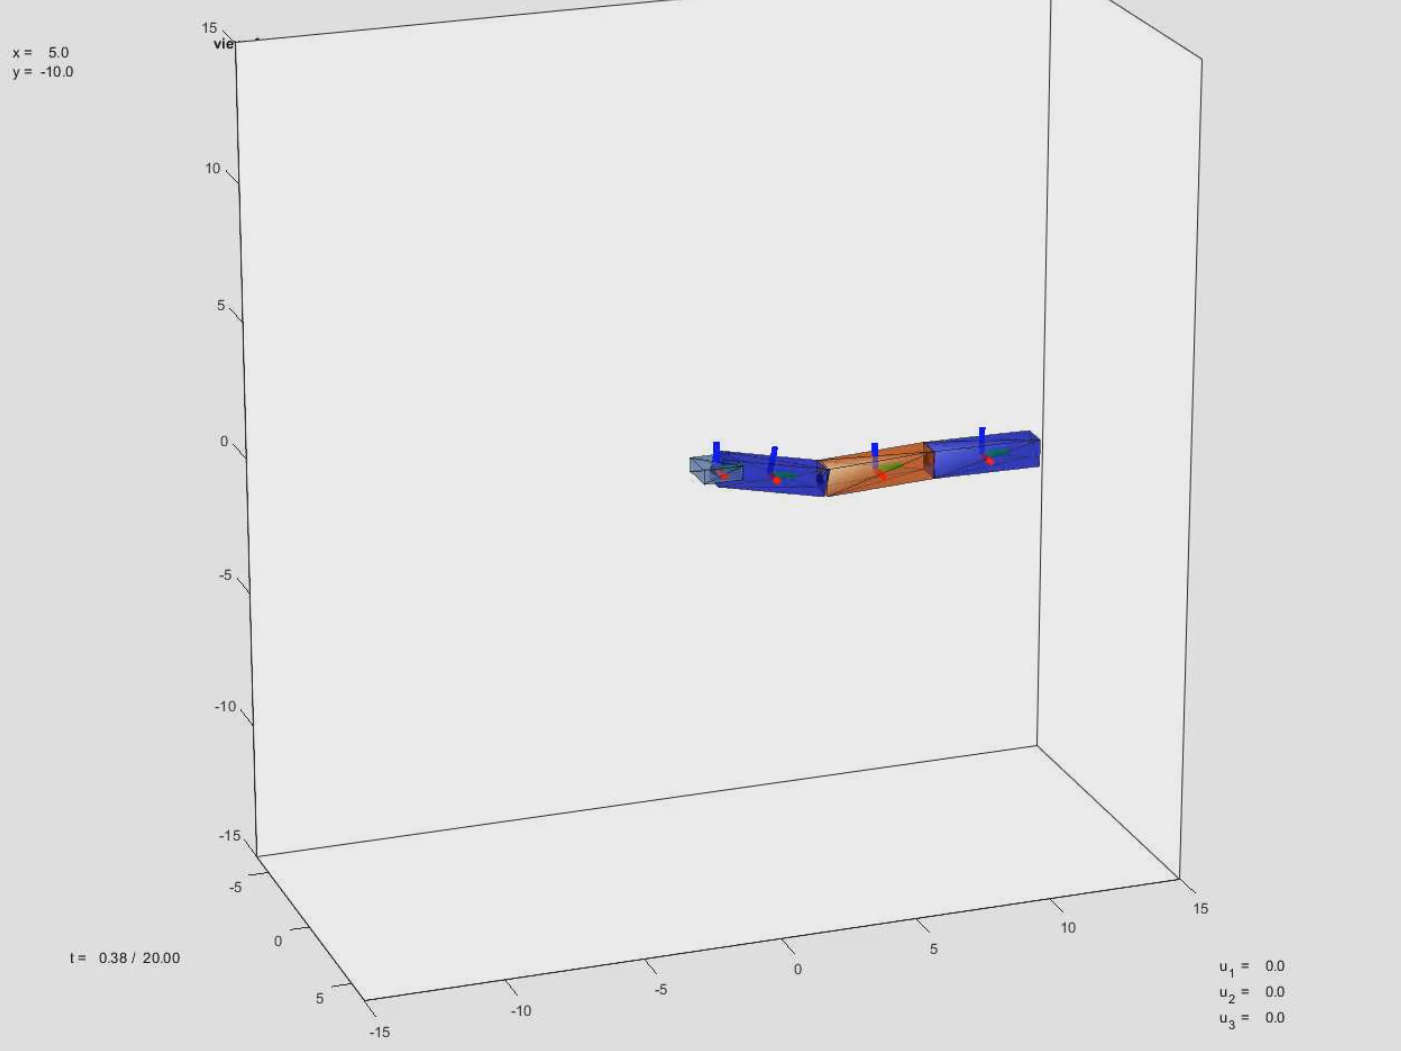
\includegraphics[scale = 0.25]{cover}}{VPlayer.swf}
\end{center}
\end{frame}

\section{Discussion}

\subsection{Full Movement Video}
\begin{frame}{Inverse Kinematics}
\begin{center}
\includemedia[activate=onclick, passcontext, transparent, addresource=movie_movement.mp4,
flashvars={source=movie_movement.mp4}
]{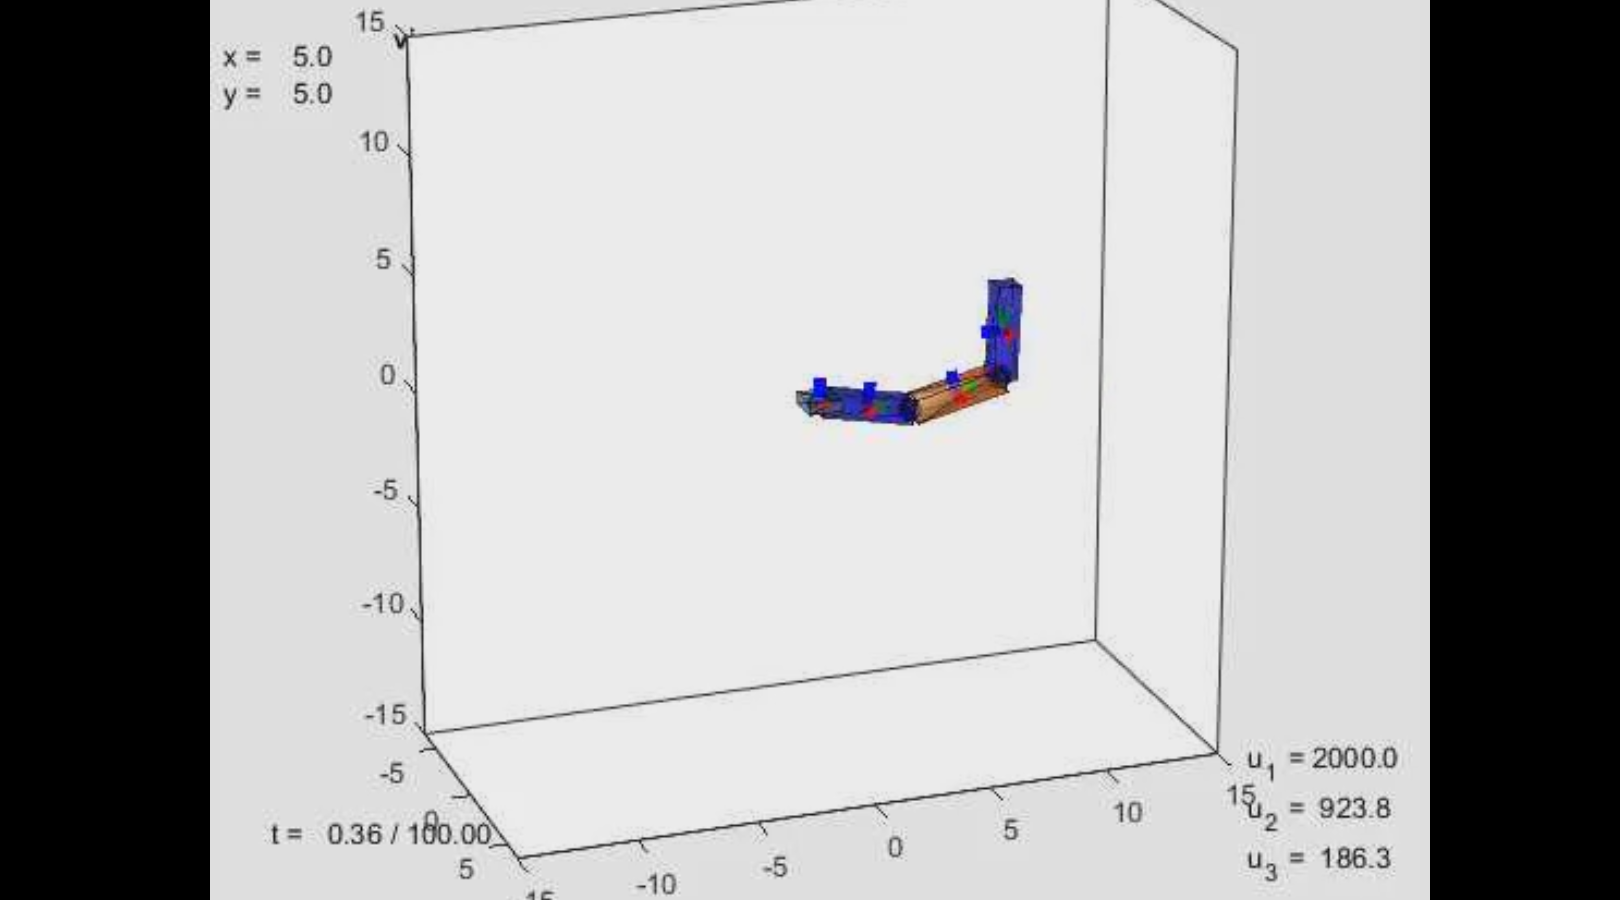
\includegraphics[scale = 0.25]{cover2}}{VPlayer.swf}
\end{center}
\end{frame}

\subsection{Questions?}
\begin{frame}
\Huge
\centering
\textbf{Questions?}
\end{frame}



\end{document}